
\begin{figure*}[htbp]
\centerline{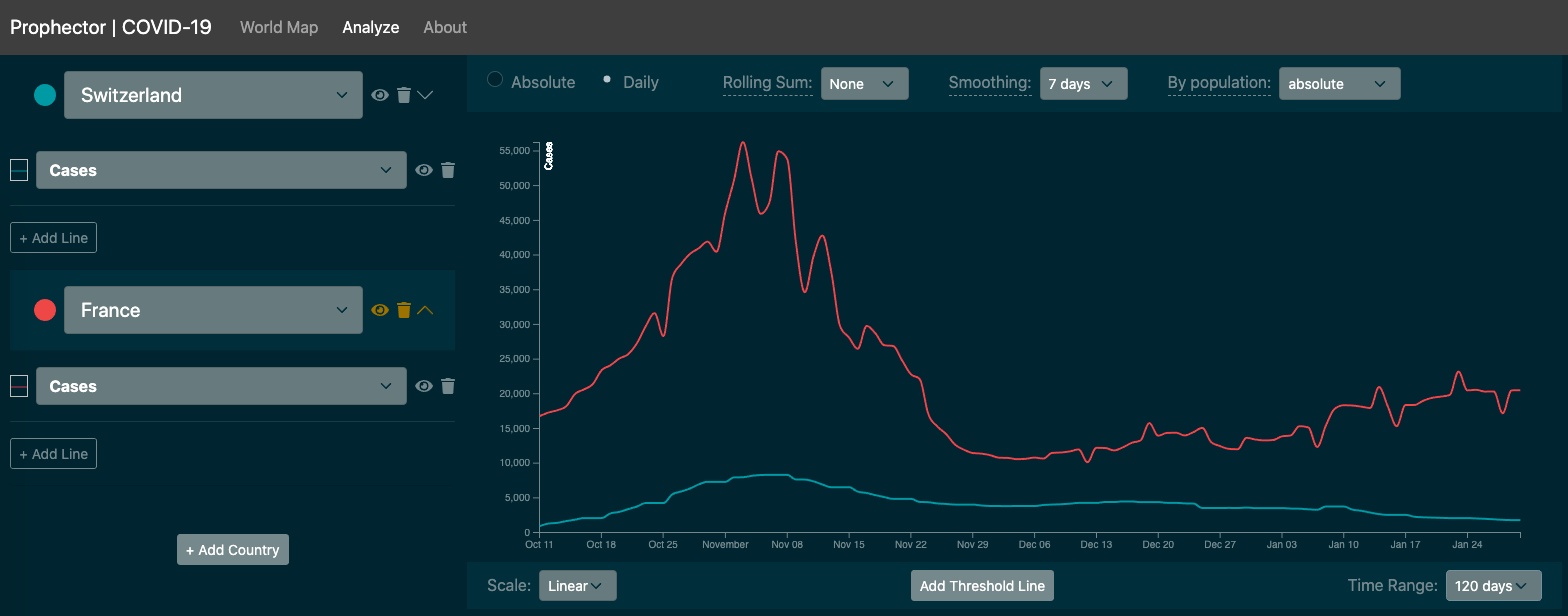
\includegraphics[scale=.328]{figs/screenshot-chart.png}}
\caption{The screenshot shows the chart analysis feature currently presenting time series data of daily cases in Switzerland and France, with a rolling mean with a window size of 7 days. The user is able to add, remove, or tweak the data selection on the left. Above the chart they can switch from absolute to daily data, change rolling sum, change rolling mean and normalization by population factors. Under the chart they can change the scale from linear to log, add a custom threshold line, and change the time frame to be shown from one to 90 days.}
\label{fig:screenshot-chart}
\end{figure*}


\section{Introduction}
The COVID-19 crisis challenges mankind in many ways and will not pass quickly, as many experts believe \cite{b6}. However, people have the desire to travel to other regions and countries within the limits of the regulations, whether for leisure or work purposes. Many countries have introduced softly defined metric-based rules for entry and quarantine restrictions. For example, the Swiss government has first defined a rule that the incidence in the last 14 days per 100,000 inhabitants of a region must be lower than 60, otherwise people returning from that area must be quarantined for 10 days. The government has since changed this rule to be relative to Switzerland's own metric. If a country has a metric 60 over the one of Switzerland, people entering from that area need to quarantine. Other countries have defined similar rules. Someone planning a vacation in the future would like to have access to the current and historic data aggregated according to these country-specific metrics, which are often not easily accessible. Additionally, they want to have a prediction of whether the country is likely to be on such a list in a few weeks.

It is trivial to find COVID-19 data \cite{b7}. That data is most often not interactively accessible for a consumer. They can download raw CSV files and write Python scripts to explore the data or they might look at charts generated by others. Many organizations and people are publishing their tables and charts online, but they don’t let one interact with them or only in a limited way.

\subsection{Combination Factor}

The combination factor is big and thus it's not possible to provide everything pre-generated. We could be interested in a combination of the following settings:

\begin{itemize}
    \item cases, tests, fatalities, vaccinations, test positivity rate
    \item country regions
    \item daily or absolute data
    \item linear or log scale
    \item rolling mean to provide curve smoothing with arbitrary window size (but most likely none, 7, 10, or 14 days)
    \item rolling sum with arbitrary window size to compute if a country-specific threshold has been surpassed or not (none, 7, 10, or 14 days)
    \item normalization by population factors (none, by 1,000,000, by 100,000, or by 10,000)
\end{itemize}

The possible amount of combinations is 244,480 assuming we have 191 countries or regions. Therefore, a practical solution lets the user define the settings they are interested in and generate the visualization on the fly. 


\subsection{Forecasting at Scale}

In the paper Forecasting at Scale \cite{b1}, Sean J. Taylor and Benjamin Letham described their solution to make the process of creating forecasts scalable in terms of limited human analyst capacity and automation. This is the approach we wanted to verify by making COVID-19 time series forecasts at scale.

With the amount of data produced and recorded by humans or machines it becomes difficult to create a forecasting model for each time series. The goal of having a super-model that can produce forecasts for any kind of time series data is very difficult to reach. We're focusing on a scalable approach that we can apply to produce reliable and high-quality forecasts for each time series separately. The challenge is the variety of time series and the lack of analysts that have expertise in their field and statistical training simultaneously. Completely automatic forecasting techniques can be hard to tune and are often inflexible to incorporate useful assumptions or heuristics. And domain experts are usually not trained in time series forecasting. This leads to a high demand for high-quality forecasts that outstrips the pace at which they can be produced \cite{b1}.

The type of scales talked about by Taylor and Letham are not computation or storage problems, as time series data usually does not have large disk requirements nor do forecasting models need a lot of computational power to be fitted today. According to the authors, scalable forecasting methods should be (1) suitable for many people, even if they have little training in forecasting, (2) suitable for a large variety of forecasting problems with idiosyncratic features, and (3) supporting efficient and automatic means of evaluation and comparing forecasts.

Once our COVID-19 time series is generated, we know the past and current state, but we would like to have a forecast of the next few days or weeks. Generating 244,480 forecasts daily is not feasible, even with Taylor and Letham's approach, in a cost effective manner, especially because most time series will likely never be looked at, and we don't know beforehand which ones those are. That's why we come to the same conclusion for forecasts as with visualizations: The user should be able to create a prediction themselves, while not requiring any statistics or programming know how. The prediction will also be displayed on their chart with \(yHat\) as well as lower and upper bounds that the fitted model generated in the backend.

This lets someone answer questions like "Can I travel to the Canary Islands in two weeks from now without having to go into quarantine upon return to my home country?".

\subsection{Justification}
A lot of solutions to the proposed problem exist already but there is still room for improvement.

Each item in this list points to an existing partial solution to the problems stated. For each item there's a justification what our solution will improve upon over the existing one.

\begin{itemize}
    \item The daily Tweets by the Federal Office of Public Health (FOPH) contain a lot of user generated statistics appended as replies.
    \begin{itemize}
        \item Our solution provides a way to explore many of the same data visualizations in an organized way with coherent design.
    \end{itemize}
    \item passportparty.ch contains blog posts with nice maps containing travel information that is unfortunately not updated daily, only contains Europe, and is not interactive.
    \begin{itemize}
        \item Our solution is capable of creating a similar geo map visualization but made interactive.
    \end{itemize}
    \item healthdata.org provides some projections which are not tweakable.
    \begin{itemize}
        \item Our solution is able to generate predictions on every type of time series (it is up to the user to decide if a prediction makes sense or not).
        \item Our solution allows a user to tweak the hyper-parameters and share them with others.
    \end{itemize}
\end{itemize}
